\section{Sviluppo}
\subsection{Modifica del \textit{database} e funzione \texttt{Login}}
Terminato lo studio delle tecnologie e del codice di {\movi} e completato il \textit{setup} dell'ambiente di 
sviluppo, ho quindi iniziato la seconda fase dello \textit{stage}, la modifica della \gls{api} di autenticazione.\\
Innanzitutto, è stato necessario aggiungere una colonna alla tabella \texttt{User} del \textit{common database}, 
che permettesse di distinguere i clienti dagli agenti. 
Nella tabella esisteva già un attributo chiamato \texttt{BPCode} (o \textit{Business Partner Code}), ovvero la chiave 
che rappresenta un cliente all'interno della propria tabella del \textit{company database}.
Ho sfruttato il fatto che gli agenti possedessero un 
\textit{id} nella loro tabella dedicata all'interno del \textit{company database} chiamato \texttt{IdUser}, 
aggiungendo questa colonna anche in \texttt{User} come chiave esterna. In questo modo ho potuto identificare come clienti 
gli utenti con \texttt{BPCode} non nullo e \texttt{IdUser} nullo, e viceversa identificare gli utenti come 
agenti.\\
Per modificare il \textit{database} ho utilizzato le potenzialità offerte da Entity Framework. In questo modo, 
mi è bastato modificare il modello delle \gls{api} e applicare le modifiche lanciando gli appositi comandi da Visual 
Studio. Aggiunta la nuova colonna alla tabella, ho provveduto a modificare un utente del \textit{database}, 
assegnandogli un \texttt{IdUser} compatibile con quelli riportati nel \textit{company database}, in modo da avere un agente 
con cui testare le nuove funzionalità.\\
Il passaggio successivo è stato modificare il servizio \texttt{UserService} al cui interno è definita la logica utilizzata 
dal \gls{api} \textit{controller} che si occupa del \textit{login}.
Inizialmente, ho nuovamente modificato il modello dei dati rendendo il \texttt{BPCode} della tabella \texttt{User} 
\textit{nullable} (cioè in grado di ammettere valori nulli). Successivamente, ho modificato la funzione \texttt{Login} e 
le relative funzioni 
di supporto, aggiungendo una serie di controlli di validità. Come ultima cosa ho testato manualmente il corretto funzionamento 
della \gls{api} e la corretta integrazione delle modifiche nel \textit{database} utilizzando Swagger.

\subsection{Sviluppo del modulo agenti}
\subsubsection{\gls{api} \texttt{GetCustomerList}}
In questa terza fase mi sono impegnato a raggiungere due obiettivi: lo sviluppo dell'\gls{api} per recuperare i clienti degli 
agenti e la creazione di una \textit{view} che chiamerò \texttt{Homepage Agenti}.\\
La \gls{api} che ho  sviluppato per il modulo agenti si chiama \texttt{GetCustomerList} e richiama all'interno del suo \textit{controller} 
la funzione chiamata \texttt{GetAgentCustomers} definita nel servizio \texttt{BpService.cs}.
Il suo funzionamento è semplice ed è il risultato finale di un processo di miglioramento continuo, in cui ho affinato il codice 
man mano che acquisivo maggiore familiarità con esso. Pertanto, descriverò solo il risultato finale, senza entrare nei dettagli 
dell'evoluzione e del ragionamento dietro lo sviluppo.\\
Una particolarità da considerare è la gestione del \textit{database} di {\movi}: il \textit{company database} è in realtà condiviso 
con un'altra applicazione, MoviSELL. La gestione e la modifica di quel \textit{database} sono quindi responsabilità di MoviSELL, 
che li ha creati e li gestisce grazie agli strumenti di Entity Framework. Per introdurre una tabella del \textit{company database} 
nel modello di {\movi}, ho dovuto lavorare al contrario, utilizzando il comando \texttt{\textit{scaffold}} di Entity Framework per costruire 
il modello a partire da una tabella esistente.\\
La tabella che avevo necessità di introdurre è \texttt{Bp}, ovvero la tabella che contiene le informazioni relative ai clienti 
aziendali. Ho utilizzato le informazioni di questa tabella anche nella funzione \texttt{Login} per controllare la validità del \texttt{BPCode} del cliente. 
Per rendere più efficiente la funzione, ho aggiunto un ulteriore valore solo per gli agenti al \textit{token} di autenticazione. 
Questo contiene al suo interno, criptate, due informazioni utili per le funzioni della \textit{Business Logic}: \texttt{CompanyCode} 
e \texttt{Username} a cui ho aggiunto il nuovo valore, l'identificativo degli agenti \texttt{IdUser}, evitando di doverlo recuperare 
nella funzione.\\
Infine, ho creato un DTO chiamato \texttt{BpCustomerDto} per ritornare i dati al \textit{controller} della \gls{api}.\\
La funzione \texttt{GetAgentCustomers} recupera due liste: quella degli utenti con \texttt{CompanyCode} uguale a quello dell'agente 
e \texttt{IdUser} nullo, e quella dei clienti con campo \texttt{IdUser} uguale a quello dell'agente (che significa in questo caso 
che il cliente è assegnato all'agente). Quindi, creo una terza lista, di \texttt{BpCustomerDto}, che contiene tutti i clienti 
appartenenti ad entrambe le liste. Questo serve ad evitare che clienti non ancora registrati nell'applicazione appaiano nella lista 
dei clienti selezionabili, oltre al fatto che sono necessari i dati presenti in entrambe le tabelle per il corretto funzionamento del modulo 
(lo \textit{username} è contenuto in \texttt{User}, mentre le informazioni come l'indirizzo del cliente sono contenute in \texttt{Bp}).

\subsubsection{\textit{Homepages}}

\begin{figure}[H]
    \centering
    \subfloat[\texttt{Homepage Agenti} definitiva di {\movi}]{
        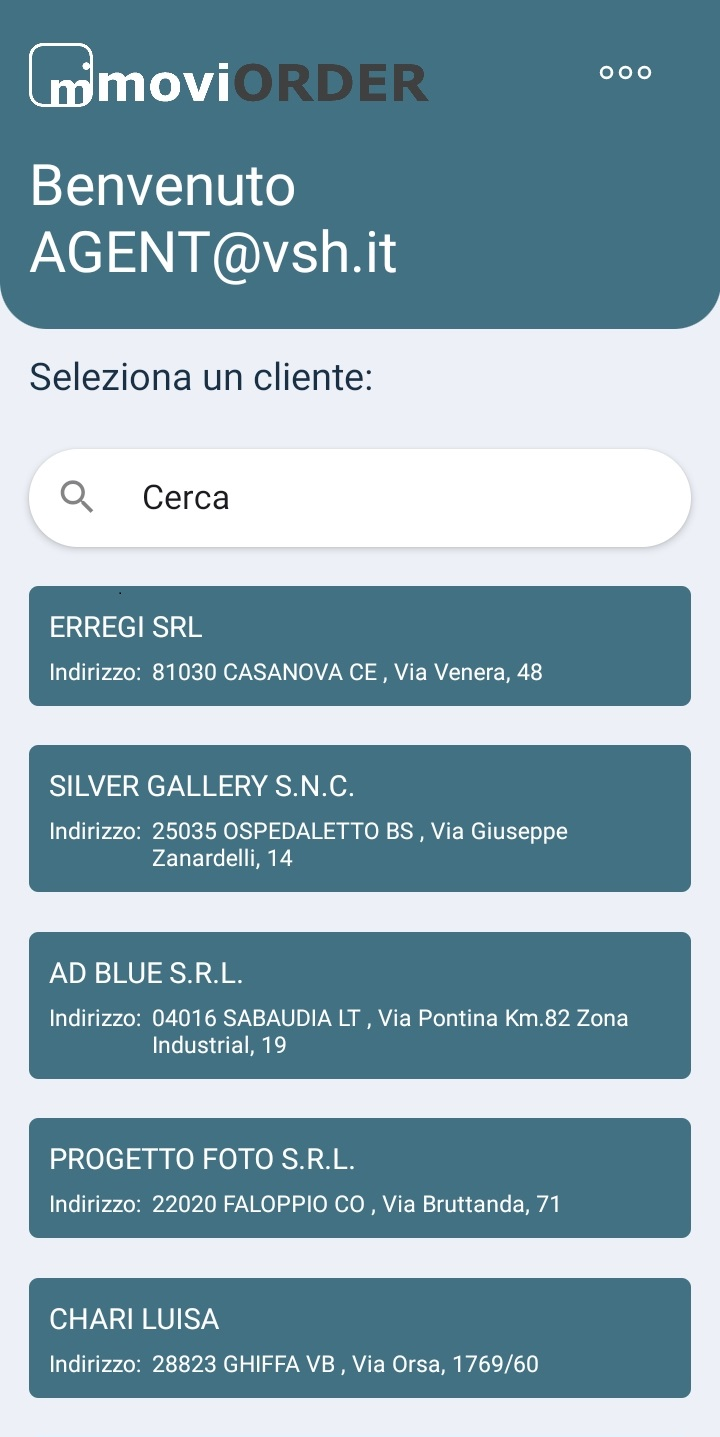
\includegraphics[width=0.3\textwidth]{img/agenthomepage.jpg}
        \label{fig:MVOR homepage}
    }
    \hfill
    \subfloat[\texttt{Homepage} definitiva di {\movi}]{
        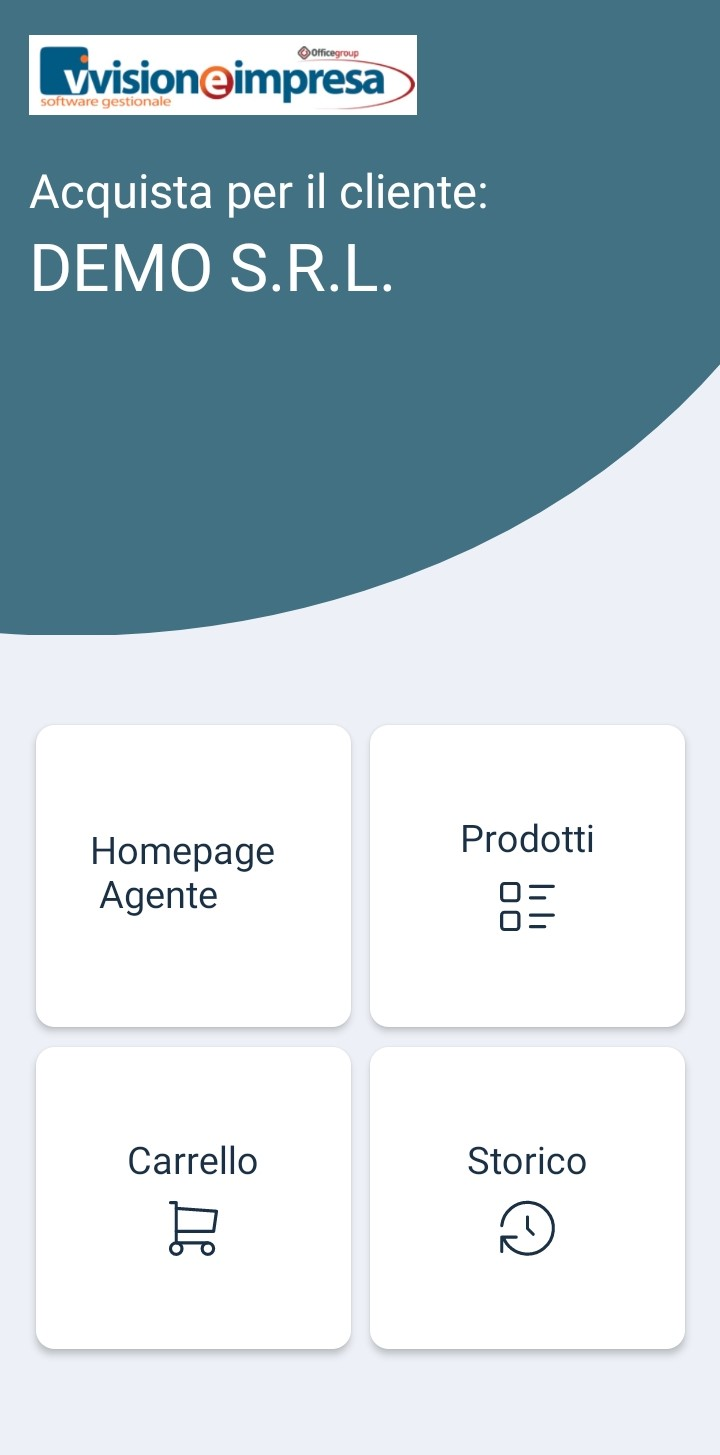
\includegraphics[width=0.3\textwidth]{img/homepage.jpg}
        \label{fig:MVOR agent homepage}
    }
    \caption{Versione finale delle \textit{homepages} di {\movi}}
    \label{fig:MVOR homepages}
\end{figure}

La nuova \textit{view} che ho creato, chiamata \texttt{Homepage Agenti}, permette agli agenti di visualizzare e 
selezionare i propri clienti. Questa \textit{view} è stata sviluppata per richiamare l'\gls{api} \texttt{GetCustomerList} 
precedentemente descritta, che consente di recuperare la lista dei clienti associati a un determinato agente.\\
A differenza dei clienti, che vengono indirizzati direttamente alla \texttt{Homepage} dopo il \textit{login}, gli 
agenti vengono invece reindirizzati alla \texttt{Homepage Agenti}. Questa \textit{view} agisce come una "camera stagna", 
in cui l'agente rimane confinato fino a quando non seleziona un cliente con cui operare all'interno dell'\textit{app}. 
Questo approccio è stato adottato per evitare che gli agenti possano cambiare la schermata senza aver selezionato 
un cliente e ridurre quindi la possibilità di comportamenti anomali. Per questo, a differenza dei clienti, ho inabilitato 
la possibilità di cambiare schermata di avvio dell'\textit{app} dalla pagina \texttt{Impostazioni}.
La figura \ref{fig:MVOR homepages} mostra le due \textit{homepage} nella loro versione finale.\\
Ho iniziato lo sviluppo costruendo la view e i \textit{component} per la lista dei clienti, in modo da poter testare il 
corretto funzionamento della \gls{api}. In questa fase iniziale, l'aspetto della \textit{view} era piuttosto grezzo e poco 
curato dal punto di vista estetico. Successivamente, ho modificato lo \textit{stack} di Navigation per rendere la \textit{view} 
visitabile, e ho aggiunto una serie di attributi specifici per gli agenti nello \textit{store} (senza tuttavia approfondirli 
in questa sede, in quanto subiranno modifiche più avanti nel processo di sviluppo).\\
Infine, ho: creato l'\textit{endpoint} per richiamare la \gls{api} \texttt{GetCustomerList}, definito un nuovo tipo chiamato 
\texttt{CustomerModel} per rappresentare i clienti che costituiranno la lista, la funzione definita nel modulo 
\texttt{Controllers} per effettuare la chiamata all'\gls{api} e i \textit{reducer} dello \texttt{Store}, 
ovvero le specifiche funzioni di Redux utilizzate per modificare lo stato dell'\textit{app}, in modo da richiamare 
la funzione del \textit{controller} in specifici momenti e in specifiche condizioni (solo se l'utente è un agente e 
solo dopo il \textit{login} o dopo l'apertura dell'\textit{app}). 

\subsubsection{\gls{api} \texttt{AdditionalLogin}}

La prima sfida che ho dovuto affrontare è stata quella di autenticare l'agente come il cliente selezionato. 
Inizialmente avevo pensato di gestire questo aspetto direttamente dal \textit{front-end}, salvando il \texttt{BPCode} 
del cliente nello \textit{store} e utilizzandolo come parametro da passare alle \gls{api}. Tuttavia, 
questo approccio avrebbe comportato la modifica di tutte le \gls{api} che recuperano il valore del 
\texttt{BPCode} usando lo \texttt{Username} contenuto nel \textit{token}.\\
Confrontandomi con gli sviluppatori di {\company} a riguardo, siamo giunti alla conclusione che questa sarebbe 
stata una scelta implementativa pessima, in quanto avrebbe compromesso l'integrità e la coerenza dell'intera 
architettura dell'applicazione.\\
Abbiamo quindi ideato una soluzione molto più semplice e pulita per risolvere il problema. Questa soluzione si basa 
sul fatto di effettuare un nuovo \textit{login} ogni volta che l'agente seleziona un cliente, utilizzando 
però una \gls{api} differente rispetto a \texttt{Login} (quella normalmente utilizzata per l'autenticazione) 
chiamata \texttt{AdditionalLogin}.\\
Questa \gls{api} funziona in maniera analoga a \texttt{Login}, ma salta tutti i controlli sulla \textit{password}. 
La sicurezza di questa \gls{api} è garantita dal fatto che per essere richiamata richiede il \textit{token} di 
autenticazione, al contrario di \texttt{Login}, garantendo che l'utente che la richiama sia un utente autenticato 
di {\movi}.\\
Questa funzione è stata sviluppata all'interno del servizio \texttt{UserService}, dove è definita anche \texttt{Login}, 
e anche per lei è stato definito un \gls{api} \textit{Controller}. 
Analogamente a \texttt{GetCustomerList}, nel \textit{front-end} ho definito la funzione che richiama l'\gls{api} 
all'interno del modulo \texttt{Controllers} e gli \textit{endpoint} nel modulo \texttt{Services}.\\
Questo approccio funziona in quanto l'\gls{api} \texttt{AdditionalLogin} ritorna gli stessi attributi restituiti 
da \texttt{Login}, incluso un nuovo \textit{token} di autenticazione. Creando le apposite variabili di supporto 
nello \textit{store} posso quindi salvare i dati del cliente e utilizzarli nell'applicazione quando necessario.\\
Per quanto riguarda la gestione dei \textit{token}, ho adottato un approccio che prevede il salvataggio di due 
\textit{token} distinti: il \textit{token} utente, che viene salvato nella memoria del dispositivo in seguito alla 
\textit{login}, e il nuovo \textit{token} ottenuto dalla chiamata a \texttt{AdditionalLogin}, che anch'esso viene 
conservato nella memoria del dispositivo.\\
Ho modificato la funzione che restituisce il \textit{token} in modo che, finché l'agente non seleziona un cliente, 
essa utilizzi il \textit{token} dell'agente. Una volta selezionato un cliente, la funzione restituirà invece il 
secondo \textit{token}, ovvero quello ottenuto dalla chiamata a \texttt{AdditionalLogin} e associato al cliente 
selezionato.\\
In questo modo, quando verranno chiamate le \gls{api}, verrà fornito il \textit{token} creato utilizzando le 
credenziali del cliente selezionato, consentendo all'agente di utilizzare l'\textit{app} come se fosse il 
cliente stesso. Questa soluzione garantisce la coerenza e l'integrità dell'applicazione, evitando di dover 
modificare le \gls{api} esistenti.

\subsection{Modifica delle interfacce}

\captionsetup[figure]{labelformat=empty, labelsep=none}
\begin{figure}[H]
    \centering
    \subfloat[\texttt{Homepage Agenti} definitiva di {\movi} per \textit{tablet}]{
        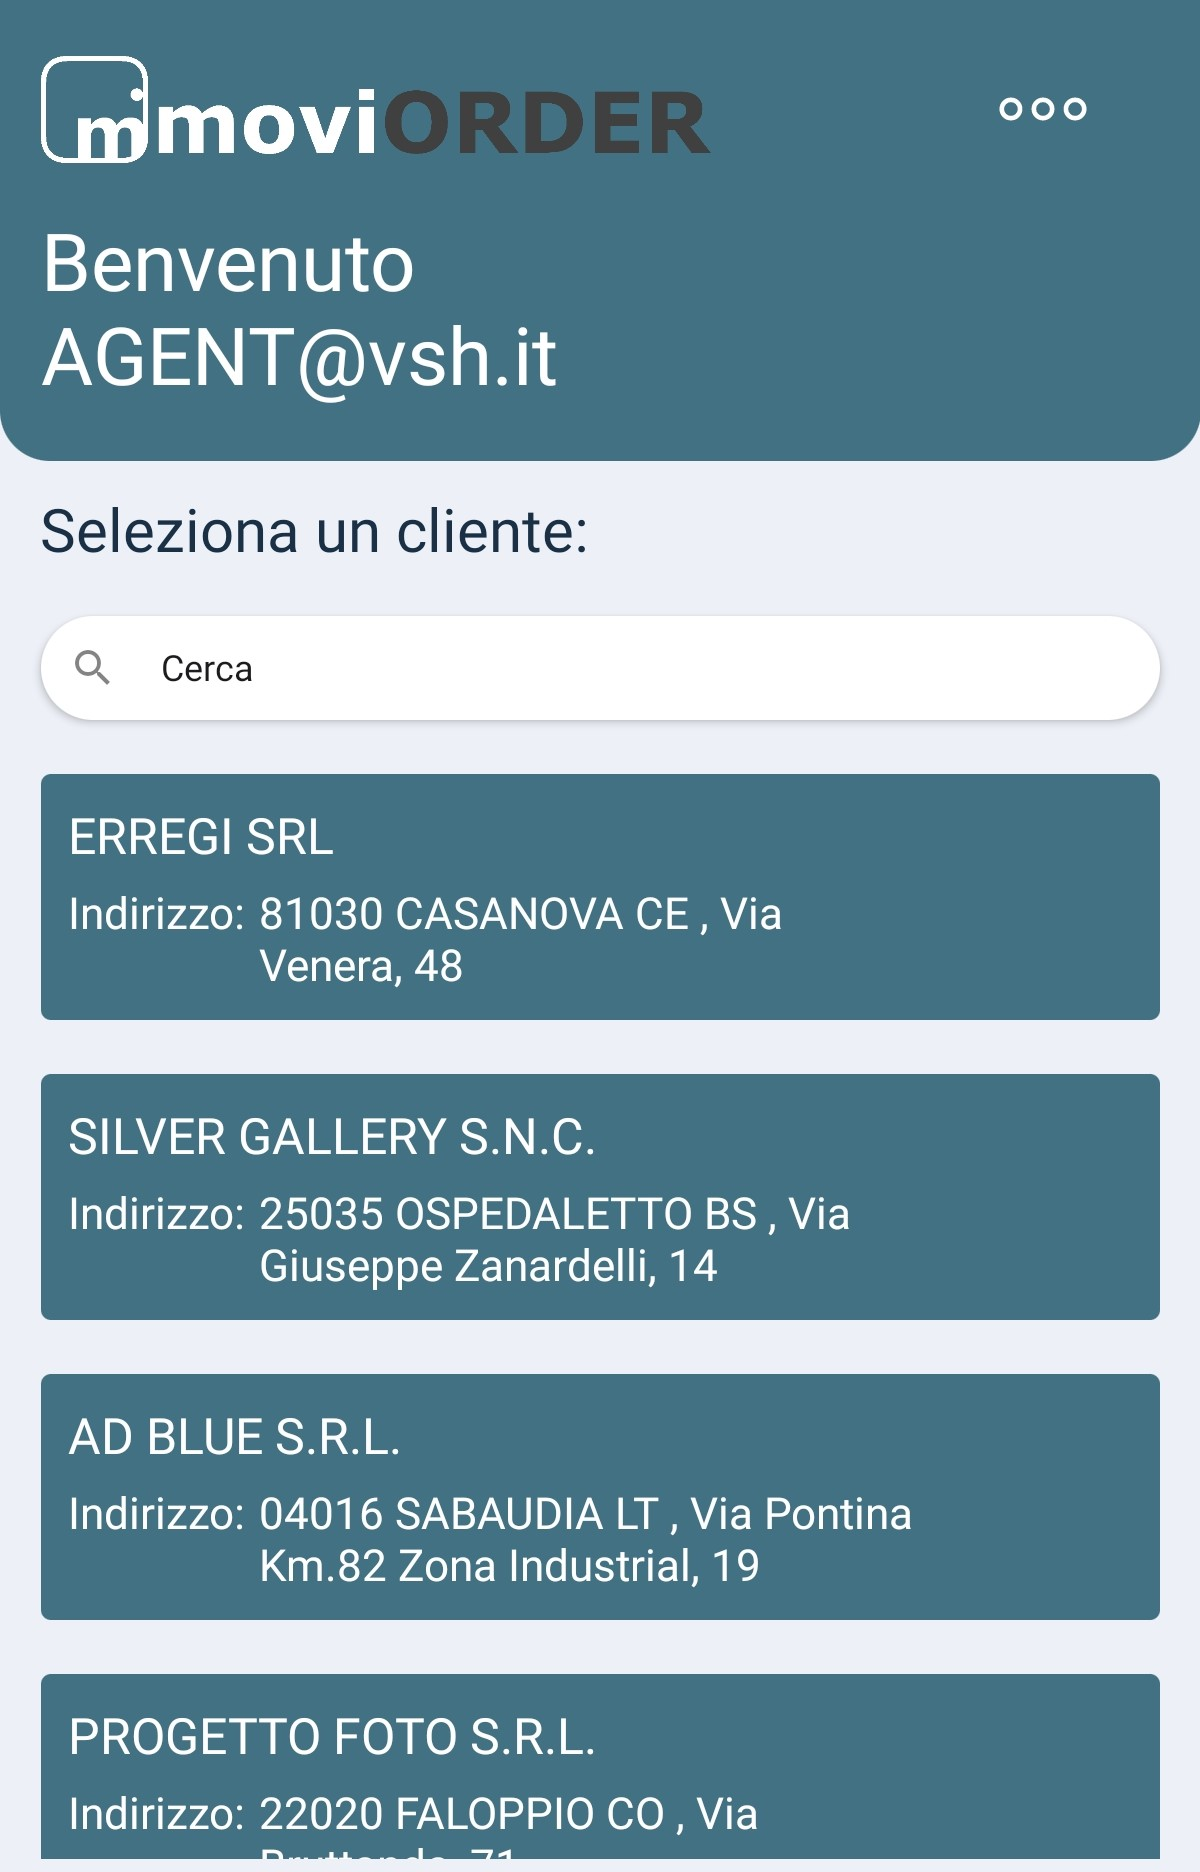
\includegraphics[width=0.35\textwidth]{img/mvor_tablet.jpg}
        \label{fig:MVOR homepage tablet}
    }
    \hfill
    \subfloat[Ricerca clienti con la \textit{search bar}]{
        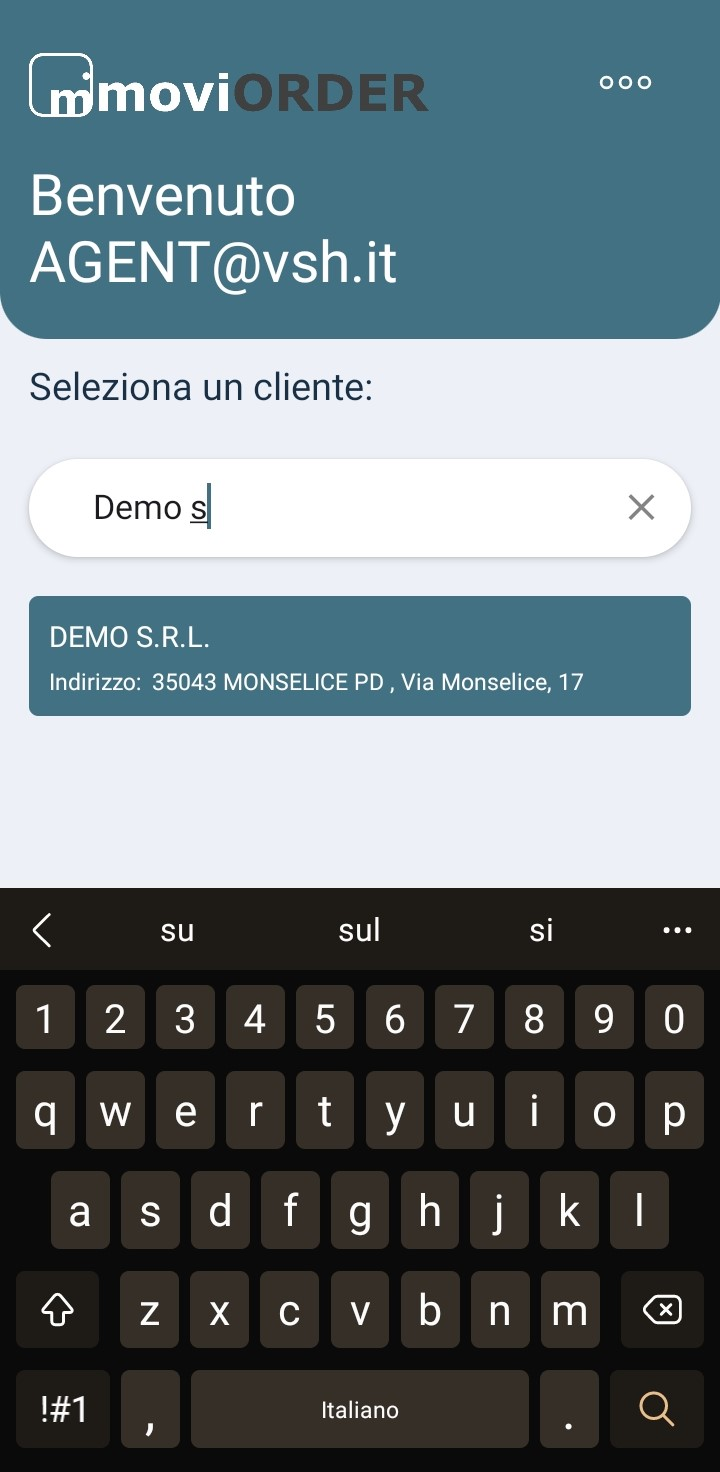
\includegraphics[width=0.27\textwidth]{img/ricerca_modulo.jpg}
        \label{fig:ricerca}
    }
    \caption[Versione \textit{tablet} di \texttt{Homepage Agenti} e \textit{search bar} 
             per la ricerca clienti nella lista]{}

    \label{fig:MVOR cose}
\end{figure}

In questa quarta fase, mi sono concentrato sulla parte grafica dell'applicazione, creando tutti i \textit{component} 
necessari (come la \textit{search bar} mostrata dalla figura \ref{fig:ricerca}) e definendo lo stile mediante l'utilizzo di CSS.\\
Per rendere i \textit{component} modulari ed indipendenti, facilitandone il riutilizzo in altre parti dell'applicazione, ho 
spostato tutta la logica di funzionamento nella \textit{view} \texttt{Homepage Agenti}. In questo modo, la 
responsabilità di ciascun \textit{component} è ben definita e separata, migliorando la manutenibilità e la scalabilità del codice.\\
Dopo aver completato questa ristrutturazione, ho apportato le ultime migliorie all'applicazione, come la possibilità di cambiare 
il tema della \texttt{Homepage Agenti} in accordo con il resto dell'applicazione. Successivamente ho adeguato il CSS 
della \textit{view} e dei \textit{component} per garantire una corretta visualizzazione anche in modalità \textit{tablet}, come 
mostrato dalla figura \ref{fig:MVOR homepage tablet}.\\
Infine, ho aggiornato i file .json che contengono la definizione delle frasi in inglese e italiano, in modo da rendere il modulo 
agenti disponibile in entrambe le lingue. Questa modifica assicura una maggiore accessibilità e inclusività dell'applicazione 
per gli utenti di diverse nazionalità.